% --- Bắt đầu SECTION: THIẾT KẾ & THỰC HIỆN ---
\subsection{Mục têu, nhiệm vụ đặt ra thực hiện đề tài}

% --- Slide 7: Kiến trúc hệ thống tổng thể ---
\begin{frame}{Kiến trúc hệ thống tổng thể}
    \begin{figure}
        \centering
        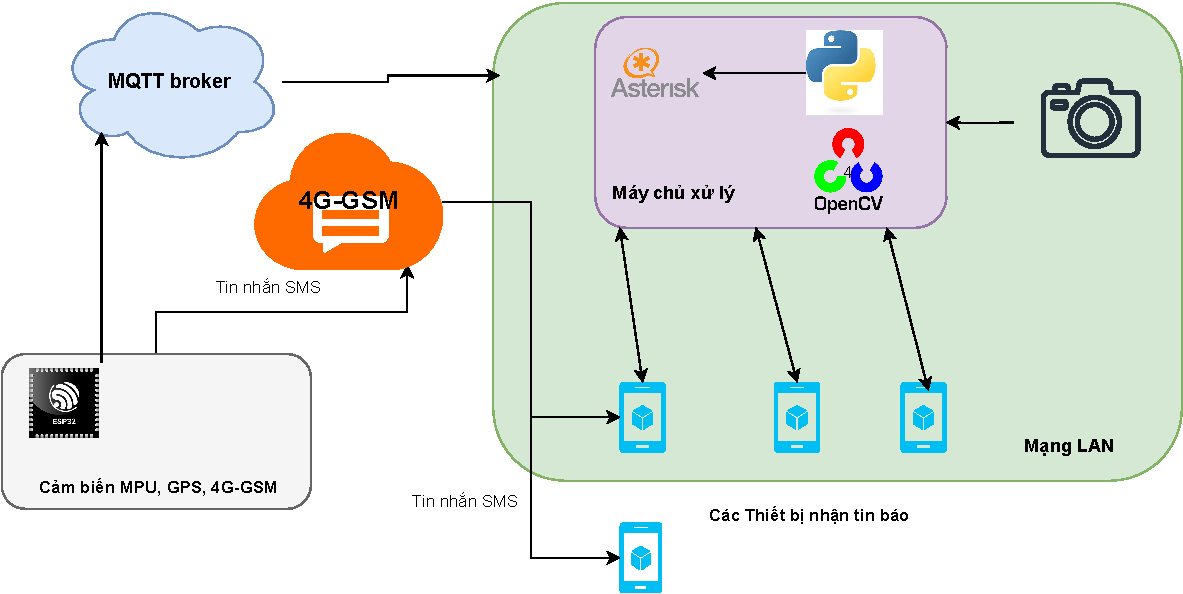
\includegraphics[width=0.8\textwidth]{images/resuilt_structure_diagram.pdf}
        \caption{Sơ đồ hệ thống tổng thể}
    \end{figure}
\end{frame}

% --- Slide 8: Hệ thống nhúng (ESP32) ---
\begin{frame}{Hệ thống nhúng (ESP32)}
    \begin{columns}[T]
        \begin{column}{0.48\textwidth}
            \begin{itemize}
                \item \textbf{Phần cứng}: ESP32, MPU6050, GPS EC800K.
                \item \textbf{Nguyên lý}: Phát hiện té ngã dựa trên ngưỡng động học.
                \item \textbf{Giao tiếp}: Gửi cảnh báo qua \textbf{MQTT và SMS}.
                \item \textbf{Ưu điểm}: Thiết bị độc lập, tiết kiệm năng lượng, dễ mở rộng.
            \end{itemize}
        \end{column}
        \begin{column}{0.48\textwidth}
            \begin{figure}
                \centering
                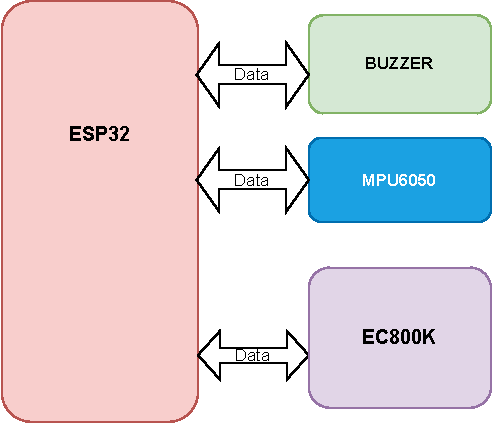
\includegraphics[width=\textwidth]{images/module1_block_diagram-crop.pdf}
                \caption{Sơ đồ nhúng ESP32 \& truyền thông}
            \end{figure}
        \end{column}
    \end{columns}
\end{frame}

% --- Slide 9: Hệ thống phân tích hình ảnh ---
\begin{frame}{Hệ thống phân tích hình ảnh}
    \begin{columns}[T]
        \begin{column}{0.48\textwidth}
            \begin{itemize}
                \item \textbf{Công nghệ}: MediaPipe, OpenCV, YOLO để trích xuất các điểm khớp xương (keypoints) và phân tích tư thế.
                \item \textbf{Quy trình}: Phân tích góc nghiêng, vận tốc, tỉ lệ khung xương để nhận diện té ngã.
                \item \textbf{Thuật toán}: Sử dụng các mô hình học máy (ML) như SVM, Decision Tree.
            \end{itemize}
        \end{column}
        \begin{column}{0.48\textwidth}
            \begin{figure}
                \centering
                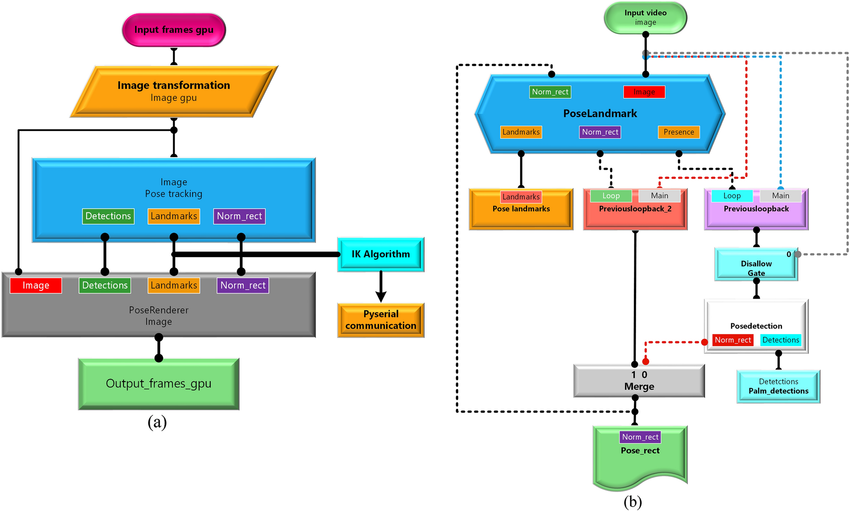
\includegraphics[width=\textwidth]{images/media_pose_pipeline.png}
                \caption{Pipeline MediaPipe + YOLO}
            \end{figure}
        \end{column}
    \end{columns}
\end{frame}

